% Inspection paradox: the gap of a Poisson process that covers a fixed time t. Generated by a short script.
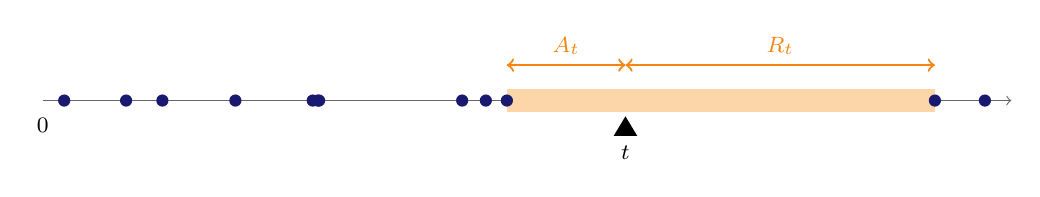
\begin{tikzpicture}[x=1cm,y=1cm,every node/.style={font=\footnotesize}]
\draw[->,black!60] (0,0)--(12.3,0);
\fill[BurntOrange!30] (5.894,-0.15) rectangle (11.330,0.15);
\draw[<->,BurntOrange,thick] (5.894,0.45)--(7.4,0.45) node[midway,above] {$A_t$};
\draw[<->,BurntOrange,thick] (7.4,0.45)--(11.330,0.45) node[midway,above] {$R_t$};
\fill[MidnightBlue] (0.272,0) circle (2.2pt);
\fill[MidnightBlue] (1.058,0) circle (2.2pt);
\fill[MidnightBlue] (1.519,0) circle (2.2pt);
\fill[MidnightBlue] (2.446,0) circle (2.2pt);
\fill[MidnightBlue] (3.428,0) circle (2.2pt);
\fill[MidnightBlue] (3.496,0) circle (2.2pt);
\fill[MidnightBlue] (3.509,0) circle (2.2pt);
\fill[MidnightBlue] (5.326,0) circle (2.2pt);
\fill[MidnightBlue] (5.627,0) circle (2.2pt);
\fill[MidnightBlue] (5.894,0) circle (2.2pt);
\fill[MidnightBlue] (11.330,0) circle (2.2pt);
\fill[MidnightBlue] (11.965,0) circle (2.2pt);
\fill[black] (7.4,-0.2)--(7.25,-0.45)--(7.550000000000001,-0.45)--cycle;
\node[below] at (7.4,-0.45) {$t$};
\node[below] at (0,-0.1) {$0$};
\end{tikzpicture}
